\chapter{リアクティブ素子とエネルギー}
\label{chap4}

第I部では，エネルギーの流れ道を高速に切り替える半導体スイッチを物理から解き明かした。
第II部では，いよいよ電力変換回路そのものに入る。
その前に，スイッチと組んで働く残りの登場人物 ― インダクタとキャパシタ ― を迎え入れる。
スイッチは流れ道を切り替えるだけで，自分ではエネルギーを蓄えられない。
切り替えの合間にも負荷へエネルギーを絶やさず届けるには，
\textbf{エネルギーをいったん蓄えて，必要なときに放出する}素子が要る。

本章では，まずスイッチだけでは電力の供給が途切れるという問題を確認し（\ref{sec4.1}節），
インダクタ（\ref{sec4.2}節）とキャパシタ（\ref{sec4.3}節）の働きをエネルギーの観点から導く。
そのうえで両者が組んで作るフィルタ（\ref{sec4.4}節）と，
周波数を変えたときのもう1つの顔 ― 共振（\ref{sec4.5}節）を学べば，
5章から始まる変換回路の解析道具がそろう。

\begin{screen}
\noindent\textbf{本章の現在地}\\[3pt]
序章の電力変換の地図（\ref{fig0.1}）でいえば，4種類の変換すべてに入る直前の入口である。
3人の登場人物のうち，本章の主役はインダクタとキャパシタ ―
\textbf{インダクタは磁場にエネルギーを蓄えて電流を保ち，
キャパシタは電場に蓄えて電圧を保つ}。
スイッチがオンの間に蓄え，オフの間に放出する。
この一往復が，これからのすべての変換回路の心臓の鼓動である。
\end{screen}

%%======================================================================
\section{なぜインダクタが電力変換の主役なのか}
\label{sec4.1}

\subsection{スイッチングは平均で電圧を作る}

序章で見たスイッチングの考え方を，まず式にしておく。
直流電圧$V_0$をスイッチで高速にオン・オフすると，
出力には$V_0$と$0$を繰り返す方形波が現れる。
オンとオフを繰り返す周期$T$を\index{すいっちんぐしゅうき@スイッチング周期}\textbf{スイッチング周期}，
その逆数$f = 1/T$を
\index{すいっちんぐしゅうはすう@スイッチング周波数}\textbf{スイッチング周波数}という。
1周期のうちオンである時間を$T_{\mathrm{on}}$とし，その割合
\begin{equation}
D = \frac{T_{\mathrm{on}}}{T}
\label{eq4.1}
\end{equation}
を\index{でゅーてぃひ@デューティ比}\textbf{デューティ比}という（$0 \le D \le 1$）。
方形波の1周期の平均電圧は
\begin{equation}
\bar{v} = \frac{1}{T}\int_0^{T} v(t)\,dt = \frac{T_{\mathrm{on}}}{T}V_0 = DV_0
\label{eq4.2}
\end{equation}
となる。
デューティ比を変えるだけで，平均電圧を$0$から$V_0$まで自在に作れる。
これがスイッチングによる電圧制御の原理であり，
抵抗で電圧を落とす方法（7章）と違って原理的に損失がない。

\subsection{平均の裏で，電力は途切れている}

しかし式\ref{eq4.2}の「平均」という言葉には落とし穴がある。
オフの期間，出力電圧はゼロであり，負荷には\textbf{電力がまったく届いていない}。
届く電力の平均値が合っていても，
照明はちらつき，モータはがたつき，ICは電源が瞬断して誤動作する。
負荷が求めているのは平均ではなく，\textbf{連続した}電力の供給である。

解決の筋道は1つしかない。
オンの間に届くエネルギーの一部をどこかに蓄えておき，
オフの間はそこから放出して穴を埋めればよい。
抵抗はエネルギーを熱に変えて捨ててしまうから，この役には立てない。
受け取ったエネルギーを蓄え，あとで回路に返せる
\index{じゅどうそし@受動素子}受動素子は，インダクタとキャパシタの2つだけである。
この2つを\index{りあくてぃぶそし@リアクティブ素子}\textbf{リアクティブ素子}と呼ぶ。

\subsection{主役はインダクタ，補助役はキャパシタ}

2つのうち，電力変換の主役を務めるのはインダクタである。
理由は単純で，負荷へエネルギーを運ぶのは\textbf{電流}だからである。
電力の供給を途切れさせないとは，電流を途切れさせないことにほかならない。
本章で見るように，インダクタは磁場にエネルギーを蓄えて\textbf{電流を保とうとする}素子である。
だから変換回路ではエネルギーが通る本流に置かれ，受け渡しの主役を務める。

一方のキャパシタは電場にエネルギーを蓄えて\textbf{電圧を保とうとする}素子である。
出力端に置かれて電圧を支え，残った変動をならす補助役に回ることが多い。
主役と補助役 ― 役割は違うが，2人は完全に対の関係（双対）にあることを
\ref{sec4.3}節で見る。

%%======================================================================
\section{インダクタ ― 磁場に蓄え，電流を保つ}
\label{sec4.2}

\subsection{素子式と磁気エネルギー}

\index{いんだくた@インダクタ}\textbf{インダクタ}は導線を巻いた素子で，
\index{こいる@コイル}\textbf{コイル}とも呼ぶ。
電流を流すと巻線の周りに磁場ができる（アンペールの法則）。
電流が変化すると磁束が変化し，電磁誘導によって巻線自身に電圧が生じる
（\index{じこゆうどう@自己誘導}自己誘導）。
生じる電圧は磁束の変化を妨げる向き，
つまり\textbf{電流の変化に逆らう向き}であり，
\index{ぎゃくきでんりょく@逆起電力}\textbf{逆起電力}と呼ばれる。

\begin{定義}[インダクタ]
\label{def4.1}
インダクタの端子電圧$v_L$は，電流$i_L$の変化率に比例する。
\begin{equation}
v_L(t) = L\,\frac{di_L(t)}{dt}
\label{eq4.3}
\end{equation}
比例係数$L$を\index{いんだくたんす@インダクタンス}\textbf{インダクタンス}といい，
単位はH（ヘンリー）$=$ V$\cdot$s/Aである。
\end{定義}

式\ref{eq4.3}はこう読む。
\textbf{電圧が現れるのは電流が変化するときだけ}である。
一定の直流に対しては$v_L = 0$，すなわちインダクタはただの導線になる。

インダクタが電流の変化に逆らうのは，磁場にエネルギーを蓄えているからである。
電流を$0$から$I$まで増やすとき，外部が注ぎ込む瞬時電力$p = v_L i_L$を積算すると
\begin{eqnarray}
W_L &=& \int p\,dt = \int L\,\frac{di_L}{dt}\,i_L\,dt
= L\int_0^{I} i_L\,di_L \nonumber\\
&=& \frac{1}{2}LI^2
\label{eq4.4}
\end{eqnarray}
となる。
これが電流$I$のインダクタが磁場の形で蓄えている
\index{じきえねるぎー@磁気エネルギー}\textbf{磁気エネルギー}である。
電磁気学で学ぶ「磁場のエネルギー密度$B^2/2\mu$の体積積分」と同じ量を，
回路の言葉で書いたものにあたる。

\begin{問}
\item インダクタンスの単位H $=$ V$\cdot$s/Aを使って，
式\ref{eq4.4}の右辺$\frac{1}{2}LI^2$の単位がJ（ジュール）になることを確かめよ。
\end{問}

\subsection{電流は急に変えられない ― エネルギー保存から}

式\ref{eq4.4}から，インダクタの最も重要な性質が導ける。
磁気エネルギー$W_L$は電流の2乗に比例するから，
もし電流が一瞬で飛び変われるなら，エネルギーも一瞬で飛び変わることになる。
有限のエネルギーを一瞬で注ぎ込む（取り出す）には無限大の電力が必要だから，
これは起こりえない。すなわち，

\begin{quote}
\textbf{インダクタの電流は連続でなければならない。}
\end{quote}

式\ref{eq4.3}の側から見ても同じ結論になる。
電流が不連続に変わるなら$di_L/dt \to \infty$，つまり無限大の電圧が要る。
インダクタは電流を保とうとし，短い時間で見れば
\textbf{一定電流を流し続ける電流源のように振る舞う}。

\begin{注意}
電流が流れているインダクタの回路を，スイッチで突然断ち切ってはいけない
（インダクタは\textbf{開放を嫌う}）。
インダクタは電流を続けようとして端子間に巨大な
\index{さーじでんあつ@サージ電圧}\textbf{サージ電圧}を発生させ，
スイッチの接点には火花（アーク）が飛び，半導体スイッチなら絶縁破壊で壊れる。
リレーやモータなど誘導性の負荷を切るときに火花が飛ぶのはこのためである。
実際の変換回路では，スイッチを切った瞬間の電流の逃げ道
（還流ダイオード）を必ず用意する。その具体的な形は5章で見る。
\end{注意}

\subsection{積分作用 ― 方形波電圧が三角波電流になる}

スイッチング回路のインダクタには，方形波状の電圧がかかる。
そのとき電流はどう動くか。式\ref{eq4.3}の両辺を時刻$t_s$から$t_e$まで積分すると
\begin{equation}
i_L(t_e) = i_L(t_s) + \frac{1}{L}\int_{t_s}^{t_e} v_L(t)\,dt
\label{eq4.5}
\end{equation}
となる。
\textbf{電流の変化は，電圧波形の面積（電圧×時間）を$L$で割ったもの}である。
インダクタは電圧を積分して電流にする素子だ，と読んでもよい。

電圧が一定値$V_0$の間，電流は傾き$V_0/L$で直線的に増える。
かけ続ければ電流は際限なく増え続ける（\FIGref{fig4.1}(a)）。
現実には巻線が焼けるか，磁性体コアが
\index{じきほうわ@磁気飽和}\textbf{磁気飽和}してインダクタとして働かなくなる。

\begin{figure}[ht]
\begin{center}
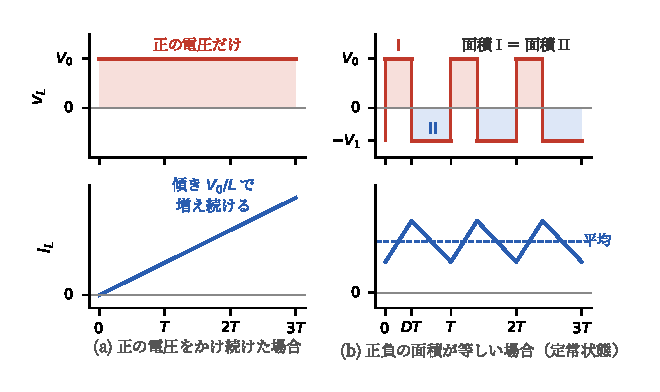
\includegraphics[clip]{figures/fig4.1.eps}
\end{center}
\caption{インダクタの積分作用。(a)正の電圧をかけ続けると電流は傾き$V_0/L$で増え続ける。
(b)正と負の電圧を交互にかけ，1周期の面積（ボルト秒）が釣り合うと，
電流は三角波を描いて同じ振動を繰り返す}
\label{fig4.1}
\end{figure}

増やしたら，減らさなければならない。
負の電圧をかければ電流は減る。
正の期間の面積と負の期間の面積がちょうど等しければ，
1周期を終えた電流は元の値に戻り，
以後同じ三角波を繰り返す（\ref{fig4.1}(b)）。
方形波の電圧が三角波の電流になる ― この波形の対応は，
5章以降の解析で何度も現れる基本パターンである。

\begin{問}
\item $L = 100\,\mathrm{\mu H}$のインダクタに$5$\,Vの一定電圧を$10\,\mathrm{\mu s}$かけた。
電流の増加分を求めよ。
\end{問}

\subsection{定常状態とボルト秒平衡}

\ref{fig4.1}(b)のように，回路の全電圧・全電流が
周期$T$ごとに同じ波形を繰り返す状態を
\index{ていじょうじょうたい@定常状態}\textbf{定常状態}という。
電源を入れた直後の過渡的な変化が収まった後の，落ち着いた運転状態である。
本書ではこれ以降，断らない限り定常状態を仮定して解析する
（序章の約束どおり，仮定はその都度明示する）。

定常状態の定義から，ただちに次の定理が出る。

\begin{定理}[インダクタのボルト秒平衡]
\label{th4.1}
定常状態では，インダクタにかかる電圧の1周期平均はゼロである。
\begin{equation}
\frac{1}{T}\int_0^{T} v_L(t)\,dt = 0
\label{eq4.6}
\end{equation}
\end{定理}

証明は1行である。
定常状態では$i_L(T) = i_L(0)$だから，式\ref{eq4.5}で左辺の変化がゼロ，
よって右辺の積分もゼロになる。
電圧×時間（単位はV$\cdot$s）の正負の面積が釣り合うことから，
\index{ぼるとびょうへいこう@ボルト秒平衡}\textbf{ボルト秒平衡}と呼ばれる。

この定理のありがたみは，
\textbf{微分方程式を解かなくても回路の電圧が決まる}ことにある。
波形の面積の釣り合いという算数だけで，変換回路の入出力関係が求まる。
5章以降に登場するすべての変換回路の解析は，この1本の式から始まる。
さっそく使ってみよう。

\begin{例題}[ボルト秒平衡で出力電圧を求める]
\label{rei4.1}
$V_0$と$0$を繰り返すデューティ比$D$の方形波電圧源に，
インダクタ$L$を介して出力をつないだ。
出力電圧は十分大きなキャパシタによって一定値$V_1$に保たれている。
定常状態における$V_1$を求めよ。
\begin{解答}
キルヒホッフの電圧則より，インダクタにかかる電圧は$v_L = v_{\mathrm{in}} - V_1$である。
すなわち
\begin{eqnarray}
v_L &=& V_0 - V_1
\qquad\mbox{（オン期間　$0 \le t < DT$）} \nonumber\\
v_L &=& -V_1
\qquad\quad\ \ \,\mbox{（オフ期間　$DT \le t < T$）} \nonumber
\end{eqnarray}
定理\ref{th4.1}のボルト秒平衡を適用すると
\begin{equation*}
DT(V_0 - V_1) + (T - DT)(-V_1) = 0
\end{equation*}
これを解いて
\begin{equation*}
V_1 = DV_0
\end{equation*}
を得る。
出力には方形波の平均電圧（式\ref{eq4.2}）がそのまま現れる。
インダクタが方形波の凸凹を受け持ち，出力へは平均だけを渡す ―
これが降圧チョッパ（5章）の原理そのものである。
\end{解答}
\end{例題}

\subsection{エネルギーバッファとしてのインダクタ}

定常状態のインダクタの働きを，エネルギーの流れで見直そう（\FIGref{fig4.2}）。
オン期間には電流が増え，磁気エネルギー$\frac{1}{2}Li_L^2$が積み上がる。
入力から受け取ったエネルギーの一部を磁場に蓄えているのである。
オフ期間には電流が減り，蓄えたエネルギーを負荷へ吐き出す。
スイッチが入力を断っている間も負荷へ電力が届くのは，この放出のおかげである。

\begin{figure}[ht]
\begin{center}
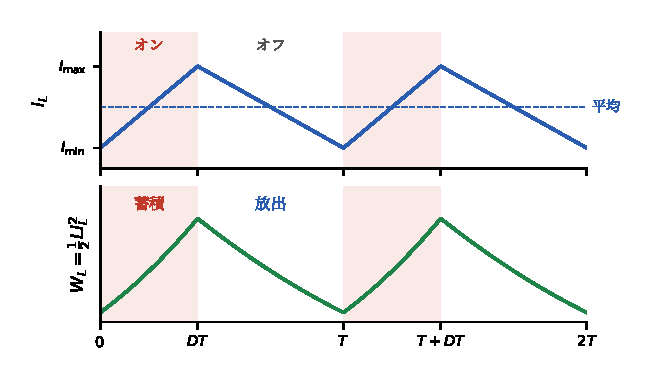
\includegraphics[clip]{figures/fig4.2.eps}
\end{center}
\caption{エネルギーバッファとしてのインダクタ。オン期間に磁気エネルギーを蓄え，
オフ期間に放出して負荷への供給の穴を埋める。定常状態では1周期の収支がゼロになる}
\label{fig4.2}
\end{figure}

蓄えて，放出する。この一往復を毎周期繰り返し，
1周期を通した収支はゼロ ― 定常状態とはそういう状態である。
エネルギーを一時的に預かって受け渡すこの役割を，本書では
\index{えねるぎーばっふぁ@エネルギーバッファ}\textbf{エネルギーバッファ}と呼ぶ。
どの素子が，いつ蓄え，いつ放出するか ―
5章以降，あらゆる変換回路をこの問いで読み解いていく。

%%======================================================================
\section{キャパシタ ― 電場に蓄え，電圧を保つ}
\label{sec4.3}

\subsection{素子式と静電エネルギー}

\index{きゃぱした@キャパシタ}\textbf{キャパシタ}は
2枚の電極で絶縁体（誘電体）を挟んだ素子で，
\index{こんでんさ@コンデンサ}\textbf{コンデンサ}とも呼ぶ。
電圧$v_C$をかけると電極に電荷$q = Cv_C$が蓄えられる。
電流は電荷の時間変化$i_C = dq/dt$だから，次の素子式を得る。

\begin{定義}[キャパシタ]
\label{def4.2}
キャパシタに流れ込む電流$i_C$は，端子電圧$v_C$の変化率に比例する。
\begin{equation}
i_C(t) = C\,\frac{dv_C(t)}{dt}
\label{eq4.7}
\end{equation}
比例係数$C$を\index{きゃぱしたんす@キャパシタンス}\textbf{キャパシタンス}といい，
単位はF（ファラド）$=$ A$\cdot$s/Vである。
\end{定義}

式\ref{eq4.7}は式\ref{eq4.3}の$v$と$i$，$L$と$C$を入れ替えた形をしている。
読み方も入れ替わる。
\textbf{電流が流れるのは電圧が変化するときだけ}であり，
一定の直流電圧に対しては$i_C = 0$，すなわちキャパシタは断線（開放）と同じになる。

蓄えるエネルギーも同じ筋道で求まる。
電圧を$0$から$V$まで上げる間に注ぎ込む電力$p = v_C i_C$を積算して
\begin{equation}
W_C = \int v_C\,C\,\frac{dv_C}{dt}\,dt = C\int_0^{V} v_C\,dv_C = \frac{1}{2}CV^2
\label{eq4.8}
\end{equation}
これが電極間の電場に蓄えられた
\index{せいでんえねるぎー@静電エネルギー}\textbf{静電エネルギー}である
（電磁気学の「電場のエネルギー密度$\varepsilon E^2/2$の体積積分」にあたる）。

\subsection{電圧は急に変えられない}

エネルギー$W_C$は電圧の2乗に比例する。
インダクタとまったく同じ論法で，電圧が一瞬で飛び変わるには無限大の電力が要るから，

\begin{quote}
\textbf{キャパシタの電圧は連続でなければならない。}
\end{quote}

キャパシタは電圧を保とうとし，短い時間で見れば
\textbf{一定電圧を保つ電圧源のように振る舞う}。
変換回路の出力にキャパシタを置くのは，
スイッチングの間も出力電圧を支える小さな電圧源を置くことなのである。

\begin{注意}
キャパシタを理想電圧源や，電圧の異なる充電済みキャパシタに直結してはいけない
（キャパシタは\textbf{短絡を嫌う}）。
電圧を一瞬でそろえようとして$dv_C/dt$が極端に大きくなり，
式\ref{eq4.7}に従って巨大な
\index{とつにゅうでんりゅう@突入電流}\textbf{突入電流}が流れる。
実際には配線の抵抗とインダクタンスで電流は有限にとどまるが，
それでもスイッチや電源を傷める。
抵抗やインダクタを直列に入れて電流を制限するのが正しい作法である。
\end{注意}

\subsection{積分作用とアンペア秒平衡}

式\ref{eq4.7}を積分すると
\begin{equation}
v_C(t_e) = v_C(t_s) + \frac{1}{C}\int_{t_s}^{t_e} i_C(t)\,dt
\label{eq4.9}
\end{equation}
となる。
キャパシタは\textbf{電流を積分して電圧にする}素子である。
積分$\int i_C\,dt$は流れ込んだ電荷（単位はA$\cdot$s $=$ C）にほかならない。
方形波の電流を流し込むと，電圧は三角波を描く（\FIGref{fig4.3}）。
\ref{fig4.1}(b)と見比べてほしい。電圧と電流の役割がそっくり入れ替わっている。

\begin{figure}[ht]
\begin{center}
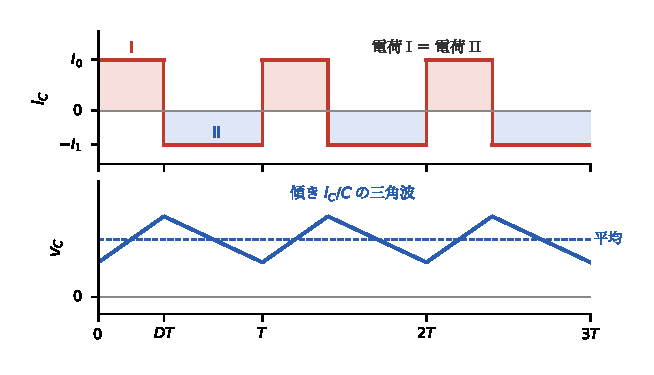
\includegraphics[clip]{figures/fig4.3.eps}
\end{center}
\caption{キャパシタの積分作用。方形波の電流を流し込むと電圧は三角波を描く。
\ref{fig4.1}(b)の電圧と電流を入れ替えた形になっている（双対性）}
\label{fig4.3}
\end{figure}

定常状態の条件も同じ筋道で得られる。

\begin{定理}[キャパシタのアンペア秒平衡]
\label{th4.2}
定常状態では，キャパシタに流れる電流の1周期平均はゼロである。
\begin{equation}
\frac{1}{T}\int_0^{T} i_C(t)\,dt = 0
\label{eq4.10}
\end{equation}
\end{定理}

定常状態では$v_C(T) = v_C(0)$だから，式\ref{eq4.9}より積分はゼロになる。
電流×時間は電荷だから，
「1周期に出入りする電荷が釣り合う」と読んで
\index{でんかへいこう@電荷平衡}\textbf{電荷平衡}とも，
\index{あんぺあびょうへいこう@アンペア秒平衡}\textbf{アンペア秒平衡}とも呼ぶ。
ボルト秒平衡と並んで，5章以降の全解析を支えるもう1本の柱である。

\begin{例題}[アンペア秒平衡で負荷電流を求める]
\label{rei4.2}
$I_0$と$0$を繰り返すデューティ比$D$の方形波電流源が，
キャパシタ$C$と負荷に並列に接続されている。
負荷には一定電流$I_1$が流れているとする。
定常状態における$I_1$を求めよ。
\begin{解答}
キルヒホッフの電流則より，キャパシタに流れ込む電流は
$i_C = i_{\mathrm{in}} - I_1$である。すなわち
\begin{eqnarray}
i_C &=& I_0 - I_1
\qquad\mbox{（オン期間　$0 \le t < DT$）} \nonumber\\
i_C &=& -I_1
\qquad\quad\ \ \,\mbox{（オフ期間　$DT \le t < T$）} \nonumber
\end{eqnarray}
定理\ref{th4.2}のアンペア秒平衡を適用すると
\begin{equation*}
DT(I_0 - I_1) + (T - DT)(-I_1) = 0
\qquad\therefore\ I_1 = DI_0
\end{equation*}
負荷には方形波電流の平均が流れる。
例題\ref{rei4.1}の電圧と電流を入れ替えただけで，答えの形まで同じである。
\end{解答}
\end{例題}

\begin{問}
\item $C = 10\,\mathrm{\mu F}$のキャパシタに$1$\,Aの一定電流を$10\,\mathrm{\mu s}$流し込んだ。
電圧の増加分を求めよ。
また，この問と\ref{sec4.2}節の問2が互いにどう対応しているか述べよ。
\end{問}

\subsection{双対性 ― LとCは鏡写し}

ここまでの結果を並べると，インダクタとキャパシタは
\textbf{電圧と電流を入れ替えた鏡写し}の関係にあることがわかる（\TABref{tab4.1}）。
この関係を\index{そうついせい@双対性}\textbf{双対性}という。

\begin{table}[ht]
\begin{center}
\caption{インダクタとキャパシタの双対性。$v \leftrightarrow i$，$L \leftrightarrow C$と
読み替えると互いに移り合う}
\label{tab4.1}
\begin{tabular}{c|c}
\hline
インダクタ$L$ & キャパシタ$C$ \\
\hline
$v_L = L\,\dfrac{di_L}{dt}$ & $i_C = C\,\dfrac{dv_C}{dt}$ \\[6pt]
磁場に蓄える　$W_L = \dfrac{1}{2}Li_L^2$ & 電場に蓄える　$W_C = \dfrac{1}{2}Cv_C^2$ \\[6pt]
電流を保つ（電流源のよう） & 電圧を保つ（電圧源のよう） \\
開放を嫌う & 短絡を嫌う \\
直流ではただの導線 & 直流では開放 \\
ボルト秒平衡（定理\ref{th4.1}） & アンペア秒平衡（定理\ref{th4.2}） \\
\hline
\end{tabular}
\end{center}
\end{table}

双対性は単なる語呂合わせではなく，実用的な思考の道具である。
片方について導いた結果は，
$v \leftrightarrow i$，$L \leftrightarrow C$，直列$\leftrightarrow$並列と読み替えるだけで，
もう片方の結果になる。
本章でもインダクタで導いた性質がすべてキャパシタで再現されたし，
5章以降でも，インダクタの電流リプルの式を導けば
キャパシタの電圧リプルの式はただちに書き下せる。

%%======================================================================
\section{フィルタとしての役割 ― 任意波形の生成}
\label{sec4.4}

\subsection{LCフィルタ ― スイッチングの跡を消す}

役者がそろったので，2人を組ませてみよう。
スイッチング電圧源のあとにインダクタを直列に，キャパシタを負荷と並列に置く。
インダクタが電流の変動を抑え，キャパシタが電圧を支える。
その結果，$V_0$と$0$を往復していた方形波は，
平均値$DV_0$のまわりにわずかな変動が残るだけの，
ほぼ平坦な直流に生まれ変わる（\FIGref{fig4.4}）。
この構成を\index{えるしーふぃるた@LCフィルタ}\textbf{LCフィルタ}，
変動をならす働きを\index{へいかつか@平滑化}\textbf{平滑化}，
残った小さな変動を\index{りぷる@リプル}\textbf{リプル}という。

\begin{figure}[ht]
\begin{center}
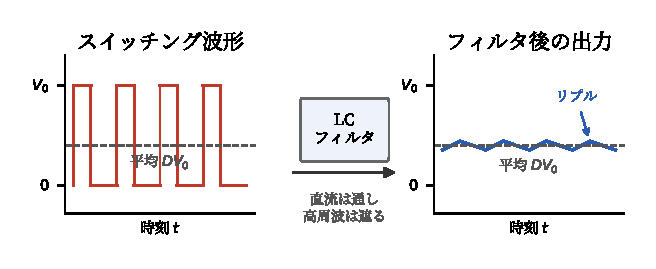
\includegraphics[clip]{figures/fig4.4.eps}
\end{center}
\caption{LCフィルタの平滑化。スイッチングの方形波から直流成分（平均$DV_0$）だけを取り出し，
出力には小さなリプルが残る。リプルは$L$，$C$を大きくするか，
スイッチング周波数を上げると小さくなる}
\label{fig4.4}
\end{figure}

リプルを小さくするには，$L$と$C$を大きくするか，
スイッチング周波数を高くして1周期に出入りするエネルギーを小さくすればよい。
「目標のリプルから$L$と$C$の値を決める」という設計手順は，5章で具体的に行う。

\subsection{周波数の言葉で言い直す}

同じことを周波数の側から見ると，フィルタの意味がはっきりする。
方形波は，直流成分（平均$DV_0$）に，
スイッチング周波数$f$とその整数倍の交流成分（高調波）を
重ねたものとみなせる。
欲しいのは直流成分だけで，残りはスイッチングが残した跡である。
LCフィルタは，直流を素通しして高い周波数を遮る
\index{ろーぱすふぃるた@ローパスフィルタ}\textbf{ローパスフィルタ}であり，
通す帯域と遮る帯域の境目の目安が
\begin{equation}
f_0 = \frac{1}{2\pi\sqrt{LC}}
\label{eq4.11}
\end{equation}
である。
$f_0$を$f$より十分低く（目安として1/10以下に）選べば，
スイッチング成分は大きく減衰し，直流成分だけが出力に現れる。
実は式\ref{eq4.11}の$f_0$はLC回路の共振周波数そのものであり，
「$f$を$f_0$に近づけてはいけない」理由も含めて，
次節でその正体を明らかにする。

\begin{問}
\item H $=$ V$\cdot$s/A，F $=$ A$\cdot$s/Vを使って，
式\ref{eq4.11}の右辺の単位がHz（$=1/\mathrm{s}$）になることを確かめよ。
\end{問}

\subsection{任意波形の生成 ― PWM}

デューティ比を一定にすれば，出力は一定の直流$DV_0$だった。
それなら，デューティ比$D(t)$を\textbf{ゆっくり変えたら}どうなるか。
出力の平均は$D(t)V_0$として追従するはずである。
たとえば
\begin{equation}
D(t) = 0.5 + 0.45\sin 2\pi f_1 t
\label{eq4.12}
\end{equation}
のようにデューティ比を正弦波状に振れば，
LCフィルタを通った出力は振幅$0.45V_0$の正弦波になる（\FIGref{fig4.5}）。

\begin{figure}[ht]
\begin{center}
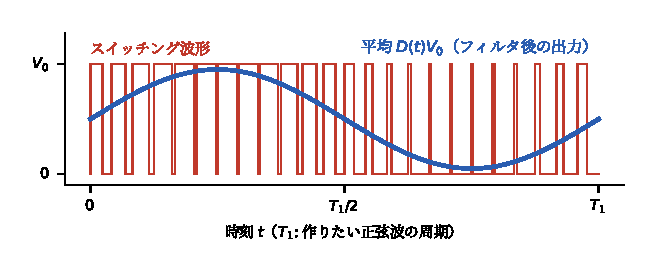
\includegraphics[clip]{figures/fig4.5.eps}
\end{center}
\caption{PWMによる任意波形の生成。デューティ比を正弦波状に変えると，
スイッチング波形の平均（＝フィルタ後の出力）が正弦波になる}
\label{fig4.5}
\end{figure}

パルスの幅で情報を運ぶこの方式を
\index{ぱるすはばへんちょう@パルス幅変調}\textbf{パルス幅変調}
（\index{ぴーだぶりゅーえむ@PWM}\textbf{PWM}: pulse width modulation）という。
直流電源とスイッチとLCフィルタだけで，正弦波でも何でも，
望みの波形が作れる ― これが直流から交流を作るインバータ（9章）の原理である。
うまく働く条件は，3つの周波数が
\begin{equation}
f_1 \ll f_0 \ll f
\label{eq4.13}
\end{equation}
と十分離れていることである
（$f_1$: 作りたい波形の周波数，$f_0$: フィルタの境目，$f$: スイッチング周波数）。
作りたい波形はフィルタを素通りし，スイッチングの跡だけが取り除かれる。

%%======================================================================
\section{共振回路とRLCのインピーダンス特性}
\label{sec4.5}

\subsection{リアクタンス ― 周波数で変わる抵抗}

前節の最後で，フィルタの働きを周波数の言葉で述べた。
これを定量的に扱う道具が，交流回路理論で学んだ複素インピーダンスである。
角周波数$\omega = 2\pi f$の正弦波に対して，各素子の
\index{いんぴーだんす@インピーダンス}\textbf{インピーダンス}は
\begin{equation}
Z_R = R，\qquad
Z_L = j\omega L，\qquad
Z_C = \frac{1}{j\omega C}
\label{eq4.14}
\end{equation}
である。
$Z_L$，$Z_C$の大きさ$\omega L$，$1/\omega C$を
\index{りあくたんす@リアクタンス}\textbf{リアクタンス}という。
抵抗と違って\textbf{周波数によって値が変わる}のがリアクタンスの持ち味である。

\begin{箇条書}
\item 低い周波数：$\omega L \to 0$（インダクタは導線），
$1/\omega C \to \infty$（キャパシタは断線）
\item 高い周波数：$\omega L \to \infty$（インダクタは断線），
$1/\omega C \to 0$（キャパシタは導線）
\end{箇条書}

LCフィルタの動作はこの2行に尽きる。
直流はインダクタを素通りし，キャパシタで堰き止められて負荷に届く。
高周波は直列のインダクタに阻まれ，
すり抜けた分も並列のキャパシタを通って逃げるので，負荷には届かない。

\begin{問}
\item H $=$ V$\cdot$s/A，F $=$ A$\cdot$s/Vを使って，
$\omega L$と$1/\omega C$の単位がどちらも$\Omega$になることを確かめよ。
\end{問}

\subsection{直列RLC回路と共振}

抵抗$R$，インダクタ$L$，キャパシタ$C$を直列につないだ回路のインピーダンスは
\begin{equation}
Z = R + j\left(\omega L - \frac{1}{\omega C}\right)
\label{eq4.15}
\end{equation}
である。
興味深いのは，$\omega L$と$1/\omega C$が\textbf{逆符号で足し合わさる}ことである。
低い周波数では$1/\omega C$が勝って容量性，
高い周波数では$\omega L$が勝って誘導性になり，
その間のある周波数で虚部がちょうど打ち消し合う。
この条件$\omega_0 L = 1/\omega_0 C$から
\begin{equation}
\omega_0 = \frac{1}{\sqrt{LC}}，\qquad
f_0 = \frac{1}{2\pi\sqrt{LC}}
\label{eq4.16}
\end{equation}
を得る。この$f_0$を\index{きょうしんしゅうはすう@共振周波数}\textbf{共振周波数}といい，
このときインピーダンスは最小値$|Z| = R$まで下がって，
回路は純粋な抵抗に見える（\FIGref{fig4.6}）。
この現象が\index{きょうしん@共振}\textbf{共振}である。

\begin{figure}[ht]
\begin{center}
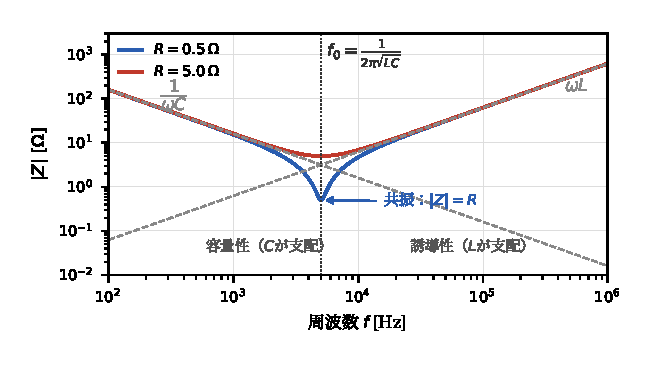
\includegraphics[clip]{figures/fig4.6.eps}
\end{center}
\caption{RLC直列回路のインピーダンスの大きさ$|Z|$の周波数特性
（$L=100\,\mathrm{\mu H}$，$C=10\,\mathrm{\mu F}$）。
低周波では$C$が，高周波では$L$が支配し，共振周波数$f_0$で$|Z|=R$まで下がる。
$R$が小さいほど谷は深く鋭い}
\label{fig4.6}
\end{figure}

共振の正体は，LとCの間のエネルギーのキャッチボールである。
電流が最大の瞬間，エネルギーはすべて磁気エネルギー$\frac{1}{2}Li_L^2$として
インダクタにあり，
電圧が最大の瞬間にはすべて静電エネルギー$\frac{1}{2}Cv_C^2$として
キャパシタに移っている。
振り子の運動エネルギーと位置エネルギーの交換と同じ構図で，
外の電源から見れば，やり取りは2人の間で完結していて，
補給が要るのは抵抗$R$で失われる分だけである。
だからわずかな電圧で大きな電流が流れ，
LやCの端子には電源電圧の何倍もの電圧が現れうる。

共振の鋭さ（\ref{fig4.6}の谷の深さ）を表す指標が
\index{きゅーち@Q値}\textbf{Q値}である。
\begin{equation}
Q = \frac{\omega_0 L}{R} = \frac{1}{R}\sqrt{\frac{L}{C}}
\label{eq4.17}
\end{equation}
$R$が小さいほど$Q$は大きく，エネルギーの交換が長く続き，共振は鋭くなる。

\begin{例題}[LCフィルタの周波数特性を数字で見る]
\label{rei4.3}
$L = 100\,\mathrm{\mu H}$，$C = 10\,\mathrm{\mu F}$，$R = 0.5\,\Omega$の直列RLC回路について，
(a)共振周波数$f_0$，(b)スイッチング周波数$f = 100$\,kHzにおける
$\omega L$と$1/\omega C$を求めよ。
\begin{解答}
(a) 式\ref{eq4.16}より
\begin{equation*}
f_0 = \frac{1}{2\pi\sqrt{100\times10^{-6}\times10\times10^{-6}}}
= \frac{1}{2\pi\times3.16\times10^{-5}} \approx 5.0\,\mathrm{kHz}
\end{equation*}
(b) $\omega = 2\pi\times10^5$\,rad/sだから
\begin{equation*}
\omega L = 2\pi\times10^5\times10^{-4} \approx 63\,\Omega，\qquad
\frac{1}{\omega C} = \frac{1}{2\pi\times10^5\times10^{-5}} \approx 0.16\,\Omega
\end{equation*}
$f$は$f_0$の20倍にあり，
スイッチング成分に対してインダクタは$63\,\Omega$の壁，
キャパシタは$0.16\,\Omega$の抜け道になる。
式\ref{eq4.13}の周波数の分離が，実際の数字でどれほど効いているかがわかる。
\end{解答}
\end{例題}

\subsection{フィルタと共振器 ― 同じLC，2つの顔}

同じ$L$と$C$の組合せでも，働かせる周波数によってまったく違う顔を見せる。

\begin{箇条書}
\item \textbf{フィルタとして}（$f \gg f_0$）：
LとCはそれぞれ電流と電圧の平滑化を静かに受け持ち，エネルギーの交換は穏やかである
\item \textbf{共振器として}（$f \approx f_0$）：
LとCが激しくエネルギーを交換し，大きな電圧・電流の振動が生じる
\end{箇条書}

フィルタとして使うときは，共振は避けるべき相手である。
スイッチング周波数やその高調波が$f_0$に近づくと，
除去するはずの成分がかえって増幅される。
負荷の急変時に出力が振動する（リンギング）のも，このLC共振の仕業である。

一方，共振をわざと利用する技術もある。
共振の正弦波振動を利用して，電圧または電流がゼロになる瞬間を作り，
その瞬間にスイッチを切り替えれば，切り替えの損失を大幅に減らせる
（ソフトスイッチング・共振形コンバータ）。
ワイヤレス給電や誘導加熱も共振の応用である。
本書の主役はフィルタとしてのLCだが，
「LとCはエネルギーを交換し合う」という本節の見方は，そうした応用の入口でもある。

これで3人の登場人物がそろった。
スイッチがエネルギーの流れ道を切り替え，
インダクタが電流を保ってエネルギーを運び，キャパシタが電圧を支える。
そして解析の柱は，ボルト秒平衡（定理\ref{th4.1}）と
アンペア秒平衡（定理\ref{th4.2}）の2本である。
次章では，この道具立てだけで最初の変換回路 ― 降圧チョッパ ― を解き明かす。

%%======================================================================
\begin{章末問題}
\item \label{ex4.1}
例題\ref{rei4.1}とは配置を変えて，
インダクタにかかる電圧が，オン期間（$0 \le t < DT$）には$v_L = V_0$，
オフ期間（$DT \le t < T$）には$v_L = V_0 - V_1$となる回路を考える。
定常状態における出力電圧$V_1$をボルト秒平衡から求め，
$V_1$と$V_0$の大小について気付くことを述べよ。

\item \label{ex4.2}
例題\ref{rei4.1}の回路（$V_1 = DV_0$）で，オン期間の電流の増加分から，
インダクタ電流のリプル（振動の幅）$\mathit{\Delta}i_L = I_{\max} - I_{\min}$が
\begin{equation*}
\mathit{\Delta}i_L = \frac{D(1-D)V_0 T}{L}
\end{equation*}
と表せることを導け。
さらに$V_0 = 12$\,V，$D = 0.5$，$f = 100$\,kHz，
$L = 100\,\mathrm{\mu H}$のときの$\mathit{\Delta}i_L$を求めよ。

\item \label{ex4.3}
例題\ref{rei4.2}の回路（$I_1 = DI_0$）で，オン期間に流れ込む電荷から，
キャパシタ電圧のリプル$\mathit{\Delta}v_C$が
$\mathit{\Delta}v_C = D(1-D)I_0 T/C$と表せることを導け。
さらに$I_0 = 2$\,A，$D = 0.5$，$f = 100$\,kHz，
$C = 10\,\mathrm{\mu F}$のときの$\mathit{\Delta}v_C$を求めよ。
この結果が章末問題\ref{ex4.2}とどう対応しているか（双対性）も述べよ。

\item \label{ex4.4}
(a) $L = 100\,\mathrm{\mu H}$のインダクタに$10$\,Aが流れているときの磁気エネルギーと，
$C = 100\,\mathrm{\mu F}$のキャパシタが$400$\,Vに充電されているときの静電エネルギーを
それぞれ求めよ。
(b) (a)のインダクタが蓄えたエネルギーを1スイッチング周期
（$f = 100$\,kHz）ごとに全部受け渡すとすると，
受け渡せる平均電力はいくらか。
スイッチング周波数を高くすると同じインダクタで大きな電力を扱える理由を，
この計算から説明せよ。

\item \label{ex4.5}
LTspiceで，$V_0$と$0$を繰り返す方形波電圧源（$V_0 = 12$\,V，$D = 0.5$，
$f = 100$\,kHz）に$L = 100\,\mathrm{\mu H}$，$C = 10\,\mathrm{\mu F}$の
LCフィルタと負荷抵抗$R = 6\,\Omega$をつなぎ，出力電圧の波形を観測せよ。
(a)出力の平均値が$DV_0$に一致すること，
(b)$C$を10倍にするとリプルがほぼ$1/10$になること，
(c)$f$を$5$\,kHz（$\approx f_0$）まで下げると出力が大きく振動することを確かめよ。
\end{章末問題}
